%% BioMed_Central_Tex_Template_v1.06
%%                                      %
%  bmc_article.tex            ver: 1.06 %
%                                       %

%%IMPORTANT: do not delete the first line of this template

%%%%%%%%%%%%%%%%%%%%%%%%%%%%%%%%%%%%%%%%%
%%                                     %%
%%  LaTeX template for BioVis 2014  %%
%%      article submissions     %%
%%          adapted from BMC    %%
%%          <8 Jan 2014>              %%
%% Liz Marai (g.elisabeta.marai@gmail.com) %%
%%                                     %%
%%%%%%%%%%%%%%%%%%%%%%%%%%%%%%%%%%%%%%%%%


%%%%%%%%%%%%%%%%%%%%%%%%%%%%%%%%%%%%%%%%%%%%%%%%%%%%%%%%%%%%%%%%%%%%%
%%                                                                 %%
%%%%%%%%%%%%%%%%%%%%%%%%%%%%%%%%%%%%%%%%%%%%%%%%%%%%%%%%%%%%%%%%%%%%%

%%% additional documentclass options:
%  [doublespacing]
%  [linenumbers]   - put the line numbers on margins

%%% loading packages, author definitions

\documentclass[twocolumn]{bmcart}% uncomment this for twocolumn layout 



%%% Load packages
%\usepackage{amsthm,amsmath}
%\RequirePackage{natbib}
%\RequirePackage{hyperref}
\usepackage[utf8]{inputenc} %unicode support
%\usepackage[applemac]{inputenc} %applemac support if unicode package fails
%\usepackage[latin1]{inputenc} %UNIX support if unicode package fails

\usepackage{mathptmx}
\usepackage{graphicx}
\usepackage{times}
\usepackage[color=yellow!30]{todonotes}
\usepackage{color,soul}
\usepackage{multirow}
%% This turns references into clickable hyperlinks.
\usepackage[bookmarks,backref=section,linkcolor=black]{hyperref} %,colorlinks
\hypersetup{
  pdfauthor = {},
  pdftitle = {},
  pdfsubject = {},
  pdfkeywords = {},
  colorlinks=true,
  linkcolor= black,
  citecolor= black,
  pageanchor=true,
  urlcolor = black,
  plainpages = false,
  linktocpage
}

 \usepackage{epstopdf}
%%%%%%%%%%%%%%%%%%%%%%%%%%%%%%%%%%%%%%%%%%%%%%%%%
%%                                             %%
%%  If you wish to display your graphics for   %%
%%  your own use using includegraphic or       %%
%%  includegraphics, then comment out the      %%
%%  following two lines of code.               %%
%%%%%%%%%%%%%%%%%%%%%%%%%%%%%%%%%%%%%%%%%%%%%%%%%


%\def\includegraphic{}
%\def\includegraphics{}



%%% Put your definitions there:
\startlocaldefs
\endlocaldefs


%%% Begin ...
\begin{document}

%%% Start of article front matter
\begin{frontmatter}

\begin{fmbox}
\dochead{Research}

%%%%%%%%%%%%%%%%%%%%%%%%%%%%%%%%%%%%%%%%%%%%%%
%%                                          %%
%% Enter the title of your article here     %%
%%                                          %%
%%%%%%%%%%%%%%%%%%%%%%%%%%%%%%%%%%%%%%%%%%%%%%

\title{A Task Taxonomy to support Visualization for the Effective Analysis of Biological Pathways}

%%%%%%%%%%%%%%%%%%%%%%%%%%%%%%%%%%%%%%%%%%%%%%
%%                                          %%
%% Do not enter the authors here for        %%
%%  a double-blind review. Otherwise        %%
%% specify information, if available,       %%
%% in the form:                             %%
%%   <key>={<id1>,<id2>}                    %%
%%   <key>=                                 %%
%% Comment or delete the keys which are     %%
%% not used. Repeat \author command as much %%
%% as required.                             %%
%%                                          %%
%%%%%%%%%%%%%%%%%%%%%%%%%%%%%%%%%%%%%%%%%%%%%%
\author[
     addressref={aff1},
  % noteref={n2},
   email={anonymous@gmail.com}
]{\inits{AA}\fnm{Anonymous} \snm{Author1}}
\author[
   addressref={aff1},                   % id's of addresses, e.g. {aff1,aff2}
   %corref={aff1},                       % id of corresponding address, if any
   %noteref={n1},                        % id's of article notes, if any
  email={alsoanonymous@gmail.com}   % email address
]{\inits{AA2}\fnm{Anonymous} \snm{Author2}}

%%%%%%%%%%%%%%%%%%%%%%%%%%%%%%%%%%%%%%%%%%%%%%
%%                                          %%
%% Enter the authors' addresses here        %%
%%                                          %%
%% Repeat \address commands as much as      %%
%% required.                                %%
%%                                          %%
%%%%%%%%%%%%%%%%%%%%%%%%%%%%%%%%%%%%%%%%%%%%%%

\address[id=aff1]{%                           % unique id
  \orgname{Anonymous}, % university, etc
  \postcode{15260}                                % post or zip code
  \city{Mariola},                              % city
  \cny{US}                                    % country
}
\address[id=aff2]{%                           % unique id
  \orgname{Anonymous Also}, % university, etc
%  \street{210 South Bouquet},                     %
  \postcode{15260}                                % post or zip code
  \city{Williamsburg},                              % city
  \cny{UK}                                    % country
}


%%%%%%%%%%%%%%%%%%%%%%%%%%%%%%%%%%%%%%%%%%%%%%
%%                                          %%
%% Enter short notes here                   %%
%%                                          %%
%% Short notes will be after addresses      %%
%% on first page.                           %%
%%                                          %%
%%%%%%%%%%%%%%%%%%%%%%%%%%%%%%%%%%%%%%%%%%%%%%

\begin{artnotes}
%\note{Sample of title note}     % note to the article
%\note[id=n1]{Equal contributor} % note, connected to author
%\note[id=n2]{Equal contributor} % note, connected to author
%\note[id=n3]{Equal contributor} % note, connected to author
%\note[id=n4]{Project leader and equal contributor} % note, connected to author
\end{artnotes}

\end{fmbox}% comment this for two column layout

%%%%%%%%%%%%%%%%%%%%%%%%%%%%%%%%%%%%%%%%%%%%%%
%%                                          %%
%% The Abstract begins here                 %%
%%                                          %%
%% Please refer to the Instructions for     %%
%% authors on http://www.biomedcentral.com  %%
%% and include the section headings         %%
%% accordingly for your article type.       %%
%%                                          %%
%%%%%%%%%%%%%%%%%%%%%%%%%%%%%%%%%%%%%%%%%%%%%%

\begin{abstractbox}

\begin{abstract} % abstract, must be under 350 words
%\parttitle{First part title} %if any
%Text for this section.

\parttitle{Background} Understanding complicated networks of interactions and chemical components is essential to solving contemporary problems in modern biology, especially in domains such as cancer and systems research.
In these domains, biological pathway data is used to represent chains of interactions that occur within a given biological process.
Visual representations can help researchers understand, interact with, and reason about these complex pathways in a number of ways.
At the same time, these datasets offer unique challenges for visualization, due to their complexity and heterogeneity.

\parttitle{Results} Here, we present taxonomy of tasks that are regularly performed by researchers who work with biological pathway data.
The generation of these tasks was done in conjunction with interviews with several domain experts in biology.
These tasks require further classification than is provided by existing taxonomies.
We also examine existing visualization techniques that support each task, and we discuss gaps in the existing visualization space revealed by our taxonomy.

\parttitle{Conclusions}  Our taxonomy is designed to support the development and design of future biological pathway visualization applications.
We conclude by suggesting future research directions based on our taxonomy and motivated by the comments received by our domain experts.


%\parttitle{Second part title} %if any
%Text for this section.
\end{abstract}

%%%%%%%%%%%%%%%%%%%%%%%%%%%%%%%%%%%%%%%%%%%%%%
%%                                          %%
%% The keywords begin here                  %%
%%                                          %%
%% Put each keyword in separate \kwd{}.     %%
%%                                          %%
%%%%%%%%%%%%%%%%%%%%%%%%%%%%%%%%%%%%%%%%%%%%%%

\begin{keyword}
\kwd{Biological Pathways}
\kwd{Pathway Visualization}
\kwd{Task Taxonomy}
\kwd{TBA}
\end{keyword}

% MSC classifications codes, if any
%\begin{keyword}[class=AMS]
%\kwd[Primary ]{}
%\kwd{}
%\kwd[; secondary ]{}
%\end{keyword}

\end{abstractbox}
%
%\end{fmbox}% uncomment this for twcolumn layout

\end{frontmatter}

%%%%%%%%%%%%%%%%%%%%%%%%%%%%%%%%%%%%%%%%%%%%%%
%%                                          %%
%% The Main Body begins here                %%
%%                                          %%
%% Please refer to the instructions for     %%
%% authors on:                              %%
%% http://www.biomedcentral.com/info/authors%%
%% and include the section headings         %%
%% accordingly for your article type.       %%
%%                                          %%
%% See the Results and Discussion section   %%
%% for details on how to create sub-sections%%
%%                                          %%
%% use \cite{...} to cite references        %%
%%  \cite{koon} and                         %%
%%  \cite{oreg,khar,zvai,xjon,schn,pond}    %%
%%  \nocite{smith,marg,hunn,advi,koha,mouse}%%
%%                                          %%
%%%%%%%%%%%%%%%%%%%%%%%%%%%%%%%%%%%%%%%%%%%%%%

%%%%%%%%%%%%%%%%%%%%%%%%% start of article main body
% <put your article body there>

%%%%%%%%%%%%%%%%
%% Background %%
%%
\section*{Background}

Understanding complicated networks of bio-molecular interactions and chemical components is essential to solving contemporary problems in modern biology, especially in domains such as cancer and systems research~\cite{hanahan2011hallmarks}.
These bio-molecular interactions are represented in the form of \emph{pathways}, which are graph models used to describe a chain of interactions between biochemical entities within a cell.
Pathways are small, curated subsets of a much larger, complex graph of interactions between molecules, and a given pathway usually represents a particular biological process, such as mitosis, that is relevant within some research context.

Pathways are modeled as labeled graphs of entities, relationships and meta-data.
For example, Figure \ref{fig:kvik} shows a typical representation of a pathway as a human-curated node-link diagram, where nodes are biological entities and edges represent interactions between them.
An entity is a component of a pathway such as a gene, a gene product (i.e. a protein), a complex of proteins, a small biomolecule within a cell, or even another pathway.
Relationships between entities can be directed or undirected, can involve multiple entites in one relationship, and can represent a wide range of biological relationships.
\hl{Meta-data can consist of experimental data, provenance information related to a particular piece of biological information, or...}
% In order to limit the scope of their analyses...

\begin{figure}[htb]
  \centering
  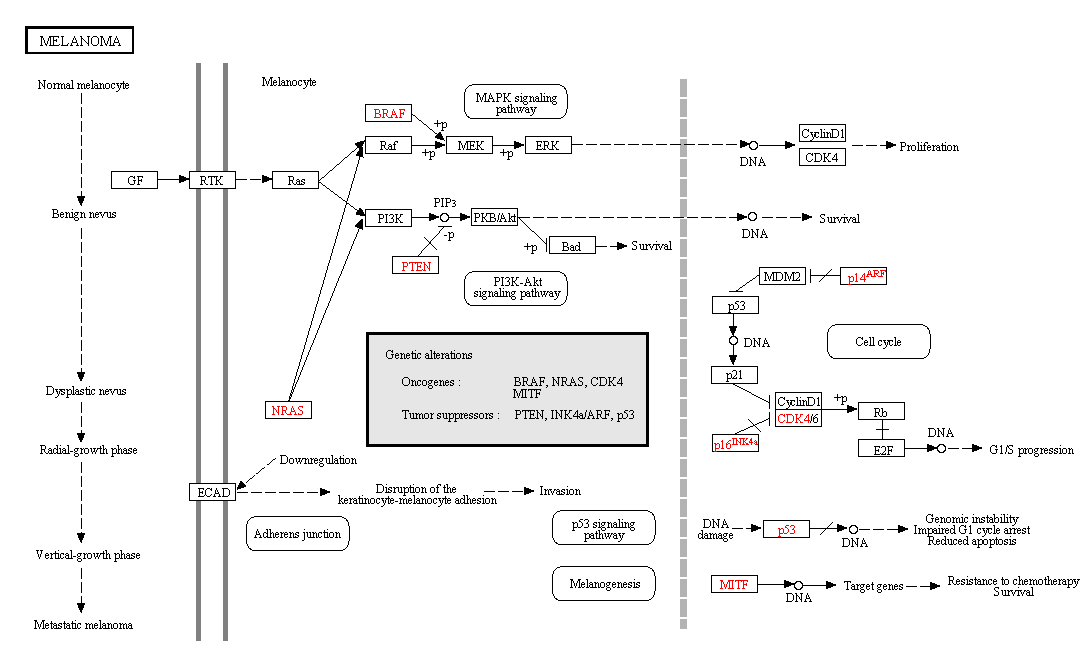
\includegraphics[width=\linewidth]{figures/kegg2}
  \caption{\label{fig:kvik} A view of a typical KEGG diagram. From~\cite{Fjukstad2014kvik}.}
\end{figure}

%\p{Pathways are very complex}

Researchers who work with pathway data are confronted with a number of challenges.
Pathway files may contain hundreds or thousands of proteins and biomolecules that participate in a variety of reactions.
\hl{Mention complexity of BioPax, and about relationships between pathways and reactions, etc.}
Participants --- genes, proteins, and other molecules within a cell --- can act as inputs or outputs to multiple reactions, and the relationships between reactions inherently include feedback loops.
Reactions often have an effect on other reactions, inhibiting or promoting their frequency.
These molecular activation pathways are inherently dynamic, which limits the utility of any static graph representation \cite{kitano2002systems}.
Representing complexity while also enabling researchers to see higher order patterns is a significant challenge \cite{saraiya2005visualizing}.

%\p{Pathways are useful for presentation}

Pathway diagrams can be useful for both presentation and analysis.
For presentation, pathway diagrams can contextualize a set of biological processes within a cell, and diagrams often show the location of cellular membranes in order to help provide a frame of reference for a given process.
Ideally, a pathway diagram allows a viewer to efficiently understand a complex set of biological relationships.

%\p{Pathways are useful for analysis}

While pathways may be useful for presenting and contextualizing a set of reactions, they can also be an important part of analyses in domains related to molecular biology and systems research, among others.
%\p{Domain context}

For example, molecular activation pathways are of critical importance to cancer researchers, who hope to understand --- and potentially disrupt --- malignant cycles of uncontrolled cellular growth, replication, and mediated cell death \cite{cairns2011regulation}.
Effective cancer drug development involves determining how proteins affected by a drug in turn affect important cellular pathways, and in this domain the downstream consequences of a particular drug effect are especially important \cite{luo2003targeting}.
In a separate domain, stem-cell researchers work with pathways that will precipitate a desired cellular differentiation into specific cell types \cite{reya2001stem}.

%\p{Static representations are not enough}

In the last decade, analyses that involve hundreds or thousands of genes and gene products have become common.
When analyzing such large and complex data, visual representations can be essential.
Often, static representations are inadequate.
The complexity and amount of information that needs to be incorporated in given diagram can make static representations cluttered and difficult to interpret.
Thus, modern tools make careful use of user interactions and visualization techniques to allow a user to effectively explore and analyze pathway data.

%\p{Designing effective tools}

Designing effective visual analytics applications requires a detailed understanding of analysis tasks that are performed by the user.
Pathway data are often large and complex, and analysts will want to perform a variety of tasks depending on their research domain.
Tasks may be exploratory in nature, and a useful visualization of pathway data could reveal new insights to a researcher.
Tasks may also involve detailed queries or calculations of various network metrics, for example.
A comprehensive understanding of tasks performed by domain researchers in a typical analysis is essential to the design and implementation of an effective visual analytics application.

%\p{Other reviews}

%Here we perform a comprehensive analysis of tasks and requirements in an effort to design effective platforms for visual analytics of pathway data.
%Previous reviews of pathway analysis tools~\cite{Gehlenborg2010omics,Suderman2007tools} have surveyed the population of available applications.
%However, the most recent review was published over five years ago, and it includes only a surface-level discussion of tasks, requirements, and visual encoding techniques.

%\p{In this work}

In this work, we present a description and analysis of tasks and requirements related to biological pathway research.
Tasks were gathered from several interviews with domain experts who work with biological pathway data.
After an introduction to the structure and content of pathway data, we describe the tasks that were garnered from our interviews.
%Using these tasks, we then describe the high-level requirements of an effective visual analytics platform for pathway data.
We then review visual representations of pathway data in the context of our requirements.
We also review existing tools that implement those visual representations.
Finally, avenues of future research are considered, along with a brief summary of lessons learned from domain experts.

%\subsection{Related Work}
%-------------------------------------------------------------------------
\subsection*{Biological Pathway Visualization}
%\todo[inline]{Need more here on history and importance}


%High throughput techniques have resulted in experiments producing vast amounts of highly complex data.
Pathways models are an important concept with biological research~\cite{cairns2011regulation, luo2003targeting,reya2001stem}.
The complexity of the data and the benefits offered to researchers by visualization tools make biological pathways an important application domain for visualization.


There are a large number of tools available and many existing surveys describe them \cite{Suderman2007tools,pavlopoulos2008survey,Gehlenborg2010omics}.
In this paper we highlight examples of prominent existing tools and techniques which provide support for the tasks described in our taxonomy, however it is not intended as a complete survey of biological visualization applications.
We have included the following: \textit{ChiBe}~\cite{Babur2010chibe}, \textit{Entourage}~\cite{Lex2013entourage}, \textit{Reactome Pathway Browser}~\cite{croft2014reactome}, \textit{VisAnt}~\cite{hu2004visant}, \textit{MetaViz}~\cite{bourqui2007metabolic}, \textit{VitaPad}~\cite{holford2005vitapad}, and \textit{BioFabric}~\cite{Longabaugh2012biofabric}.
It is clear from the relationship structure of pathway data that graphs are a suitable visualization choice, and each of these applications visualizes pathway data as node-link graph representations (or a slight variant in the case of Biofabric~\cite{Longabaugh2012biofabric}.
Cytoscape \cite{cytoscape} is a graph visualization application which is designed for biological data, and also offer’s many plugins for visualizing pathway data, such as Cerebral\cite{Barsky2008cerebral} and RenoDoI\cite{Vehlow2015}.
However, there are alternative visualization techniques which could be applied to pathway data.
Research has shown that matrix visualization techniques outperform node-link diagrams for higher level group based tasks\cite{Ghoniem2004,Henry2007}.
While matrix tasks are not as effective for path-tracing tasks, a juxtaposition of both types or a hybrid visualization hybrid, such as NodeTrix~\cite{NodeTrix2007}, could prove effective.
% mention Set visualization




\subsubsection*{Pathway Data Formats}
Pathway data can be stored in one of several file formats.
In particular, \textit{BioPAX}~\cite{demir2010biopax}, \textit{KEGG}~\cite{kanehisa2000kegg} and \textit{SBML} \cite{Hucka2003} are the most popular standards for storing the complex data structures described in the previous section.

These formats are XML-based and represent data as an ontology.
\emph{BioPAX}, in particular, was designed to be a general format for biological pathways across a variety of domain contexts~\cite{demir2010biopax}.
Systems Biology Graph Notation (SBGN)~\cite{Novere2009} is a visual standard often used to visualize \textit{BioPAX} and \textit{SBML} file formats.
This standard defines multiple edge and node types, as well as allowing edges to connect to more than 2 nodes, resulting in a hypergraph visualization.
Other formats are employed for the visualization of biological pathways that are not specific to the field of biology.
For instance \textit{SIF Simple Interaction Format} used by \textit{Cytoscape}~\cite{Shannon2003cytoscape} is used to visualize undirected interactions between participants.

%However, the most recent review was published over five years ago, and it includes only a surface-level discussion of tasks, requirements, and visual encoding techniques.



%-------------------------------------------------------------------------
\subsection*{Task Taxonomies}
The field of visual analytics has produced a number of \textit{task taxonomies}, which are written in an effort to understand exactly how various analytics tasks are enabled by different visualization techniques, and vice-versa.
These taxonomies help clarify the utility of existing techniques while also providing a low level template for the design and evaluation of new techniques.
Wehrend and Lewis~\cite{Wehrend1990} provide one of the earliest visualization task taxonomies, with the goal of ``accelerating progress in scientific visualization'' by allowing researchers to easily find the right visualization technique for a given problem.
Schneiderman~\cite{Shneiderman1996} define a ``task by data type taxonomy'' for information visualization in order to \textit{``to sort out the prototypes and guide researchers to new opportunities''}.
These seminal taxonomies were, like many later taxonomies, independent of a specific visualization application domain, their purpose was to provide a low level description and categorization of the analysis tasks enabled by \textit{any} visualization of data.

Later taxonomies focus specifically on more narrow categories of visualization.
For instance, Valiati et al.~\cite{Valiati2006} provide a taxonomy focused specifically on multidimensional visualizations. They build on~\cite{Wehrend1990}, but focus on tasks uniquely related to multidimensional visualizations (such as parallel coordinates).
Like previous authors, their goal is to guide the choices of visualization and interaction techniques, and also to  help support usability testing.
Lee at al~\cite{Lee2006} define a graph visualization taxonomy of tasks that are frequently encountered when analyzing graph data.
The stated goal of this work was to improve the evaluation of graph visualization systems by creating a set of common benchmark tasks (which could be used in conjunction with benchmark data sets).
Their taxonomy covers tasks for the analysis of graphs in general, and was inspired by example tasks from many domains that make regular use of graph data.
The authors build on Amar and Stasko's~\cite{Amar2005} low level visual analytic task list by composing existing low level tasks into higher level complex tasks while also proposing additional tasks that are not captured by low level tasks presented in existing taxonomies.


Several recent taxonomies focus on aspects of graph visualization that extend the work of Lee at al~\cite{Lee2006}.
Ahn et al~\cite{Ahn2014} provide a task taxonomy for analyzing networks that evolve over time, also known as dynamic graphs.
The dynamic and complex nature of dynamic graph data yields a similarly complex set of analysis tasks, and many of these tasks are not covered by the general graph taxonomy of Lee at al~\cite{Lee2006} -- thus, new tasks need to be specified.
Pretorius et al~\cite{Pretorius2014} focus on multivariate graph visualization (where graph elements contain multiple attributes).
Their work builds on the work of both Lee at al~\cite{Lee2006} and of Valiati et al.~\cite{Valiati2006}, as multivariate networks can be considered a multidimensional data set.

The earliest visualization taxonomies were written as very general classifications of low level analytic tasks related to any data visualization.
In more recent publications, and as visualization research has progressed, task taxonomies have increasingly focused on more constrained subsets of tasks related to particular types of data structures.

While recently-published task taxonomies have focused on particular data structures (or for datasets with particular characteristics), to our knowledge this is the first written in the context of the domain of biological pathway analysis.

\todo[inline]{One could argue that the whole point of a taxonomy is to be general, and to ignore domain. We should highlight the benefits of writing a taxonomy based on domain-specific tasks. Or how this interesting... etc.}

Biological Pathway visualization is a complex application domain that poses many specific challenges not encountered in the created of the previous taxonomies
The underlying data sets are dynamic multivariate hyper-graphs, and are more complex than any of those described in previous taxonomies.
The tasks to be completed by biologists are also highly complex, involving many different entity and relationship types, and are not fully covered by the existing taxonomies.
\todo[inline]{Need to demonstrate 100 percent that this is true in the rest of the paper}
%Amar and stasko do include correlation as one of their tasks
% pretorius also includes causation...

%-------------------------------------------------------------------------






\section*{Methods}
\subsection*{Interviews}
Interviews were conducted with seven biological scientists, each of whom works with pathway data in some form.
Those interviewed included one tenured professor, three assistant professors, one researcher at a cancer research institution, one postdoctoral research associate, and one masters student in bioinformatics.
Interviews were loosely structured, but interview questions were designed to elicit a detailed understanding of the tasks performed by the researcher in a typical analysis, as well as an understanding of the type and structure of data that each researcher worked with.
Each researcher also presented their views on the utility of pathway data and pathway diagrams in general.
We have develop a full task taxonomy based on these interviews. 
In addition to this, we describe examples of how tasks are handled by current biological visualisation applications, we shown how the tasks could be address using contemporary grpah and information visualization techniques.



%\begin{figure}[t!]
  %\centering
  %\includegraphics[height=3.5in]{placeholder.eps}
  %\caption{Example two-column figure. To insert a single column figure, remove the * in the two figure tags. }
  %\label{fig:interface}
%\end{figure}


\section*{Results and Discussion}

%\section{Task Taxonomy}

\begin{table*}
  \begin{tabular}{| l | l |}
    \hline
    \multirow{2}{*}{Attributes} & Provenance \\
    & Uncertainty \\ \hline
    \multirow{5}{*}{Relationships} & Directed \\
    & Hierarchical \\
    & Compound \\
    & Cascading \\
    & Feedback Loops \\ \hline
  \end{tabular}
\end{table*}

% \subsection{Taxonomy Overview}

Biological pathways are represented as weighted, directed, labeled graphs which can include hyper-edges and compound nodes.
While task taxonomies exist \hl{citation} which describe tasks related to the visual analysis of graphs in general, the analysis of bio-molecular interaction networks reveals several important graph-analytic tasks that other works have not described in detail. This taxonomy refines and extends the existing set of tasks associated with the visual analysis of network data.

\subsection*{Attributes}

The low-level identification of nodes, edges, and their attributes is an essential component in the visual analysis of any graph representation.
In the context of biology, this task is complicated by the fact that the attribute of an edge can itself be a complex object.
Here, we highlight three forms of attribute data that are particularly relevant to biological contexts: multivariate data from experimental results, provenance data, and measures of uncertainty.
We also discuss the need for the integration of external data sources.

\subsubsection*{Multivariate Attributes}

\paragraph*{Description}
The entities within a biological pathway can contain many attributes that reflect the state of a biological entity in a given context, experimental condition, and time.
For example, each biomolecule in a particular pathway can be associated with gene expression levels across several different experimental conditions, and each of these conditions can include an additional temporal dimension~\cite{Barsky2008cerebral}.
In this case, each node in a graph is associated with at least three additional dimensions of experimental condition, expression level, and time.
This multivariate data can also apply to relationships between entities, such as when one gene is up-regulated or down-regulated by another gene under different experimental conditions.
This change in attributes may be time based (meaning the graph is dynamic) or it may be as a result of the context in which a pathway is being analyzed (e.g. as part of a cancer research study).

% Data entities containing multiple attributes are often referred to as multivariate.

% \subsubsection{Multivariate Attributes: Techniques}
\paragraph*{Existing Approaches and Techniques}
Multivariate network visualization is a highly active field of visualization, in which the life sciences in general are frequent application domain, see \cite{} for a recent state of the art survey.
Many more recent biological network visualizations include attribute information.
CHiBE \textit{ChiBE}\cite{Babur2010chibe} provides the ability to load in biological entity regulation data mappings from an external source and apply them to a pathway visualization.
The most prominent data format for supporting this is the SIF format defined as part of the Cytoscape application \cite{Shannon2003cytoscape}.
The \textit{RenoDoI} application \cite{Vehlow2015}, a plug-in for \textit{Cytoscape}for visualizing biological data knowledge networks, uses Degree of Interest functions to highlight nodes based on attribute values.
Such functionality could easily be extend to biological pathway visualizations.
The general purpose visualization system , \textit{Candid} \cite{Shadoan2013}, also uses attribute information as part of hyper graph query system which allows users to perform complex queries on entities of different types.
Node and edge attributes are also used for graph querying and filtering as came be seen in , what is termed \textit{facet} based visualization. This approach allows for graphs to be filtered by subsets of attributes.

\todo[inline]{need to include Cerebral application here}
The cerebral application uses attribute information as an aid to layout. The graph layout space is divided into layers and nodes are positioned in the layers based  on sub-cellular localization annotation, essentially an attribute of the node.
%To Be Completed

\subsubsection*{Provenance}

\paragraph*{Description}
Especially important to researchers in the field of bioinformatics is the concept of \textit{data provenance}, which refers to the history of original sources tied to a particular entity.
Much of the data in the field of bioinformatics is gathered and integrated from a wide range of publications, data stores, and other products of research.
Information related to a single entity can be based on potentially dozens of different publications that have been produced across a wide range of time.
For example, each relationship within a BioPAX file is usually associated with a publication that provides evidence for its existence.
The task of visually identifying provenance is complicated in two ways.
First, each piece of research related to a given biological entity may corroborate, extend, or contradict earlier publications.
Second, the biological context under which a particular entity is studied often varies.
The individual studies related to a given gene or gene product might have incorporated cells taken from a variety of tissues, organs, and species.
Thus, the provenance information related to a given biological entity can be seen as a temporal network of provenance data, with each publication being tied to earlier works in a variety of ways.

\paragraph*{Existing Approaches and Techniques}
While \textit{SBGNViz}~\cite{SBGNViz2015} and \textit{ChiBE}\cite{Babur2010chibe} and other applications allow connectivity to external sources, such as UNitProt or TBA, provenance information is not visualized directly.

% Does it need to be
% \todo[inline] {Discuss Visualization of provenance}

\subsubsection*{Uncertainty}

\paragraph*{Description}
Related to the task of identifying data provenance is the task of being able to view and identify information related to the \textit{uncertainty} of the data underlying entities and the relationships between them.
The importance of understanding uncertainty was emphasized by several of the researchers we interviewed.
Uncertainty may relate directly to the provenance history discussed above -- biological entities that are related to more recent research may have a limited set of one or two publications which corroborate their functionality, while other genes and gene products may have a rich history of robust empirical evidence from dozens or hundreds of publications.
An even more fine-grained approach to uncertainty visualization could somehow incorporate the uncertainty or error tied to individual empirical findings.
The empirical support behind any individual entity or relationship within a pathway can vary widely, and the question of how these varying levels of confidence can be incorporated into a pathway visualization has been rarely addressed.

\paragraph*{Existing Approaches and Techniques}
Some databases such as STRING~\cite{STRING2005} , a protein interaction database, provide quality scores with their results. This quality score can be seen as a form of uncertainty based on the provenance of the data.
The higher the score, the more evidence there is for an interaction.

\subsection*{Relationship Tasks}
Bioinformatics is, essentially, the study of relationships between biological entities, and understanding relationships within a biological pathway graph is one the most essential tasks that a systems biologist will perform.
All of the researchers we interviewed stressed the importance of understanding how pathway entities within a biological network are connected.
Here, we discuss some of the complex types of relationships found within biological datasets.
We emphasize that the challenge of visualization is not that these different categories of relationship exist, but that they exist as combinations and compositions of each other. \hl{work on wording}

\subsubsection*{Multivariate Relationships}

\paragraph*{Description}
As discussed above, one of the most obvious challenges for biological network visualization is the fact that the types of relationship between entities are numerous, and even hierarchical.
For instance, an interaction between two entities could take many forms, including: the binding of proteins and molecules into complexes, the translocation of an entity from one cellular location to another, a change in gene expression activity, or the modification of existing compounds, to name a few. 
Each of these events can be further specified. 
A modification can take many forms, such as \textit{ubiquitination} or \textit{phosphorylation}, and the \textit{site} at which these modifications occur can also be specified.
Changes in gene expression are directional -- one compound can either \textit{increase} or \textit{decrease} the activity of another.
A translocation event will typically specify \textit{from} and \textit{to} locations.
Thus, not only are there many different types of relationship (and generally more than can be effectively encoded using color alone), but each relationship type has its own set of potential specifications, some of which can be quite detailed.
The visual encoding of these complex and multivariate relationships is one of the more prominent challenges in the design of visual analytic platforms for biological pathway analysis.
\begin{figure}[htb]
  \centering
  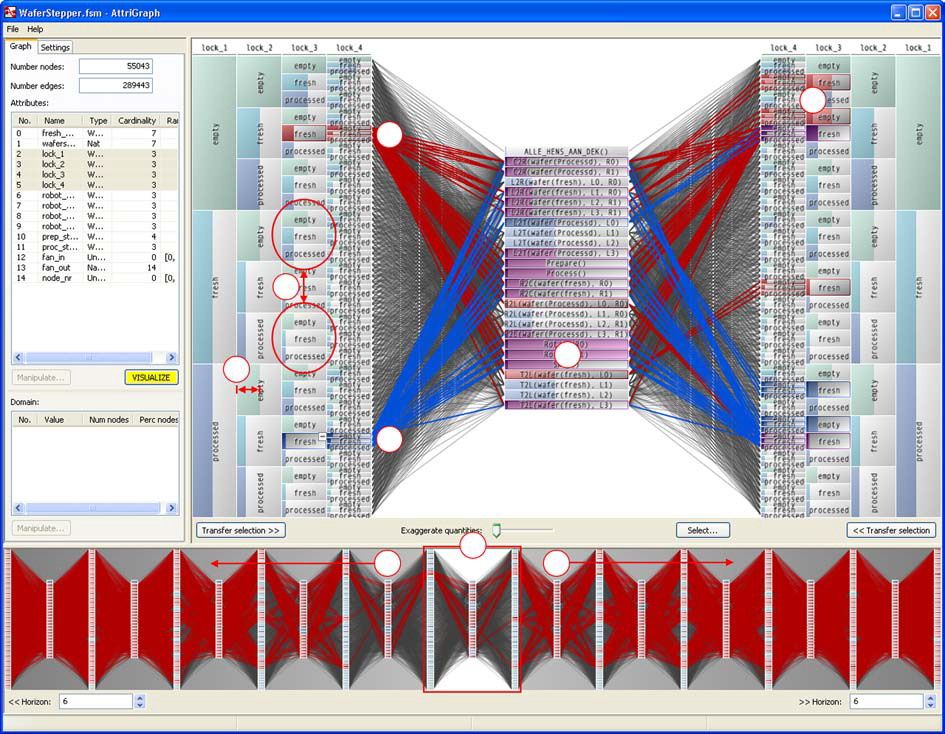
\includegraphics[width=0.95\columnwidth]{figures/MultivariateViz}
  \caption{\label{fig:MultivariateViz} Screen shot taken form Pretorius and Van Wijk's~\cite{pretorius2008} multivariate graph visualization application. Permission to be obtained. }
\end{figure}

\paragraph*{Existing Approaches and Techniques}
Pretorius and van Wijk's~\cite{pretorius2008} system for visual inspection of multivariate graphs places relationship type (referred to as edge labels) at the core of their system.
They do not use traditional graph layout techniques. 
The edges are grouped by label in the center of the display, nodes are duplicated on either side, with the attributes reflected by an icicle plot (see figure \ref{fig:MultivariateViz}).
This approach can handle a large number of edge types, and cases where a node is involved in multiple relationships of different types.

Ghani et al~\cite{Ghani2013} developed a techniques called Parallel Node-Link Bands (PNLBs) for exploring graphs with multiple edge types. In their examples edge types are inferred based on their endpoint node types. Nodes are listed in vertical columns with  the edges connecting only between neighboring columns.
Is is similar to Pretorious and van Wijk's approach except there are multiple columns of nodes and there is only ever one type of edge between two columns. It is an effective visualization, but is generally limited to smaller data sets and  those in which the relationship types are multiple bimodal relationships (as there are no edges drawn between non-adjacent columns).
\hl{to-do Create stonger relationship between this paragrap and the previous}

\subsubsection*{Directed Relationships}

\paragraph*{Description}
While some analyses and datasets involve undirected relationships between genes or gene products, the majority of studies of metabolic networks and other inter-cellular processes rely on directed relationships. 
Several researchers that we interviewed stressed the importance of understanding directed relationships between entities.
Depending on the type of relationship in question, edges may be \textit{bi-directional}, which is distinct from an \textit{undirected} edge.
A visual coding that indicates direction must also be able to account for cases in which there are two directional edges between the same two nodes.
\begin{figure}[htb]
  \centering
  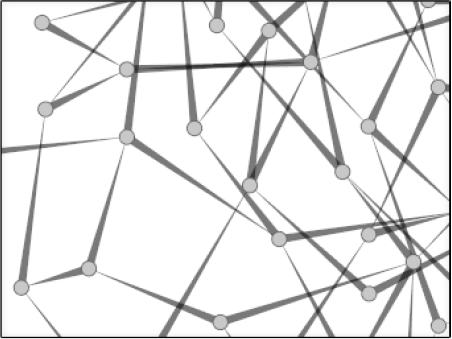
\includegraphics[width=0.8\columnwidth]{figures/tapered_edges}
  \caption{\label{fig:tapered_edges} The tapered directional edges, taken from~\cite{Holten2009}. Permission to be obtained. The narrow end of the edge indicates the target.}
\end{figure}

\paragraph*{Existing Approaches and Techniques}
Many visualization applications use the more traditional approach of arrowheads to indicate edge directions, however work by Holten and van Wijk~\cite{Holten2009} shows that tapered edges (see fig \ref{fig:tapered_edges}) perform more effectively in conveying edge direction. The graphs used in Holten and van Wijk's were simple directed graphs. Biological pathways are usually modeled as hyper-graphs, with many different types of edge and hyper-edge. Visual encodings such as SBGN and KEGG (see figure \ref{fig:kvik}) contain many different visual representations for edges, so applying the tapered edge visualization style to complex biological pathways is not trivial and would require an empirical evaluation. However, the results of Holten and van Wijk's work suggest that investigating such an approach may be worthwhile.

\subsubsection*{Hierarchical Relationships}

\paragraph*{Description}

Pathway data is inherently hierarchical.
Hierarchical relationships describe relationships of containment, and these relationships can be abstract or based on real biochemical interactions within a cell.
For example, a pathway (itself an abstraction) can be nested within other pathways.
These nested pathways generally encapsulate some commonly-understood hierarchy of biological processes that take place within a cell, such as cellular replication.
Other representations include the more general notion of a ``module'' of connected components, such as gene products.
Hierarchical relationships can also represent physical interactions between biochemical participants.
A common of example of this is in bio-molecular complexes, which are themselves composed of other complexes or biomolecules.

It is important to note that hierarchy and ``structure'' often co-exists with other types of relationships. In most cases, pathway data includes relationships of hierarchy (i.e., when one vertex is contained within another) \textit{in parallel} with other, non-hierarchical relationships, such as the relationship between one gene product that activates or inhibits another. Also, note that while non-hierarchical relationships can take a variety of forms, the only form of hierarchical relationship is one of \textit{containment}, from parent to child, and is undirected.
\begin{figure}[htb]
  \centering
  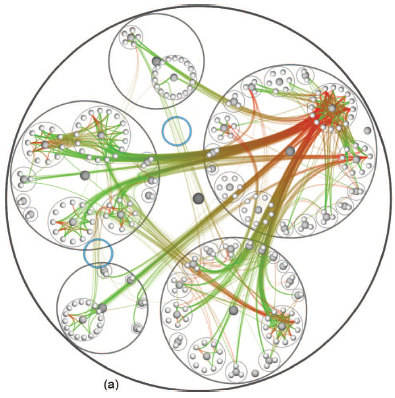
\includegraphics[width=0.5\columnwidth]{figures/Hierarchical_edge_bundles}
  \caption{\label{fig:Hierarchical_edge_bundles} Hierarchical edge bundles, taken from~\cite{Holten2006}. Permission to be obtained. The bundles not only reduce clutter but also more cleary define the hierarchy.}
\end{figure}

\paragraph*{Existing Approaches and Techniques}
In terms of visualization there are many techniques for showing hierarchical data.
There are many hierarchical tree based graph layouts that position nodes to emphasis hierarchical nature of data, however these are often not suitable for biological pathway layout as the constrains on position in a layout affect the readability of the lowest level of information.
The RenoDoI application allows for multiple data sources to be included in a single diagram.
This may include data from different pathways and is a containment relationship. Essential the node for each data source forms a set, which may or may not overlap with other sets.
This is visualized using by drawing a bounded contour around the nodes in the set. Different border colors indicate different sets.
This type of encoding of  set membership is the \textit{Bubblesets}~\cite{Collins2009} approach, which was shown to be the most effective way of displaying group information on a node link diagram by Jianu et al.~\cite{Jianu2014}.
\todo[inline]{consider moving previous paragrap to compound Relationships section}




In many cases for pathway visualization the hierarchy is not very deep and edges do not traverse multiple levels of the hierarchy.
However in cases where edges do traverse  multiple hierarchical levels they may cause clutter.
Hierarchical Edge Bundling \cite{Holten2006} is a clutter reduction technique, which also emphasizes the hierarchical nature of relationships, see figure\ref{fig:Hierarchical_edge_bundles}. There are many edge bundling techniques in general, however most do not respect hierarchical information during routing.

\subsubsection*{Compound Relationships}

\paragraph*{Description}

A vertex that contains other entities can be represented as a \textit{compound node}, which is equivalent to a ``parent'' vertex or in some contexts a ``module.''

It is important to note that a one-to-one relationship between an entity and a parent is \textit{not} the same as a one-to-many relationship between an entity and all of that parent's children.
For instance, the \textit{BioPax} format allows for the abstract ``NextStep'' relationship, which defines, as the name suggests, an arbitrary notion of the ``next step'' of some biological process.
A biochemical reaction could be connected, via a \textit{single} ``NextStep'' relationship, to an entire pathway, which could potentially contain thousands of nodes.
This relationship is clearly not the same as a biochemical reaction being connected to every entity within a pathway.
This example also demonstrates the distinction between a compound relationship and a hierarchical relationship.
A connection from a node to a compound node does not imply a relationship of ownership or containment.

\paragraph*{Existing Approaches and Techniques}

\hl{to-do}

\subsubsection*{Causality and Cascading Effects}

\paragraph*{Description}

% \todo[inline, author=PM]{Should we separate discussion of cause and effect from discussion of cascading effects?}
A category of tasks inherent to a variety of work in bioinformatics is the identification of \textit{causal relationships} that exist between bio-molecular entities, and \emph{causal networks} are of particular importance to the analysis of large-scale gene expression data.

When discussing directed paths between entities, one entity is said to be \emph{upstream} or \emph{downstream} of another.
For example, one gene product can increase the activity of other gene products that are \emph{downstream} of it.
Understanding these upstream and downstream relationships is particularly important to domains such as cancer drug research, where a drug may affect a small subset of genes or gene products, which in turn will affect various downstream processes.
In most cases, a directed relationship is meant to represent a biochemical reaction, where one entity is consumed as a reactant and another is produced as a product.
Thus, an upstream entity may be connected to a downstream entity through a chain of several directed links, and a researcher may be interested in understanding the path of reactions (or other relationships) that connects two entities.
However, most cellular processes are inherently complex, and involve many competing sets of directed interactions.
Any given gene is often \textit{mediated} by many different reactants, some which increase activity, and others which decrease activity.
For instance, a causal network helps reveal the likely regulators of a set of genes that are observed to be up-regulated or down-regulated in a particular setting~\cite{felciano2013predictive, Kramer2013ipa-causal}.

Thus, determining the set of entities that are "responsible" for the increase or decrease in the expression of a particular gene is a challenging task that involves a complex array of directed relationships between many upstream entities.
We characterize this problem as one of identifying \textit{cascading effects}, where many upstream entities have directed relationships with many mediating entities, which in turn affect the output of many downstream entities.

\paragraph*{Existing Approaches and Techniques}

Archambault and Purchase~\cite{Archambault2016} have performed a empirical evaluation of different techniques for showing attribute cascades.
They found that visually small multiples was the best approach to convey the dynamic attribute changes that cascade through a network.
The small multiples approach is a form of comparative juxtaposition where multiple views of the network at different time points are displayed in a matrix.
This approach has been used by the cerebral application for showing cascades of data.
Archambault and Purchase's work also shows that layout has an impact on the visualization of attribute cascades.
Experiment participants performed better when a hierarchical layout was used, however it should be noted that the hierarchical layout was consistent with the direction of the layout.

\todo[inline, author=FMG]{I think it would be a good idea to differentiate this taxonomy from Ahn's taxonomy in this section. He does look at causal tasks and repetition, which are related to feedback loops , but not the same....}

\subsubsection*{Feedback Loops}

\paragraph*{Description}

In tandem with the problem of identifying cascading effects is the problem of reasoning with feedback.
Feedback loops are common within metabolic activation networks, and they play a key role in processes related to uncontrolled cellular growth in cancerous cells.

\paragraph*{Existing Approaches and Techniques}

\hl{to do}

\subsection*{Comparisons}

\paragraph*{Description}

Related to the issue of multivariate attributes is the need to compare related pathways or sets of entities, or to compare a given pathway across a number of states.
For instance, microarray measurements are often used to measure gene expression levels for a control group and an experimental group over several time steps.
The goal of this research is to discover significant empirical differences between groups and across time, and the visual comparison of these groups is useful.

\paragraph*{Existing Approaches and Techniques}

In their 2011 survey Gleicher et al. \cite{Gleicher2011} describe three primary types  classifications of comparative visualization.
These are  juxtaposition, superposition,  and explicit encoding of differences, and these classifications can also be combined.
Juxtaposition is when the visualizations being compared are displayed side by side.
This is functionality is available by default in Cytoscape ( and hence all of the associated plug-ins).
Cerebral uses a juxtaposition approach to display changes in attributes associated with the graph.

Superposition is when is when data sets are displayed as part of the same visualization.
The RenoDoI plugin also offers superposition , allowing multiple networks to be  visualized in the  one image. Bounding isocountours are used to distinguish graphs differences, and to clearly indicate where the graphs overlap.
Graph layout is and important aspect of both juxtaposition and superposition based comparative visualizations.
For juxtaposition, the two graphs being compared should have as similar layout in possible , to aid comparison.
For supposition, the matter is not so simple as the addition of a new graph may destroy the existing layout.
The RenoDoI application\cite{Vehlow2015} initially lays out the largest data set, then adds the addition data sets, adjusting previous layout , without resetting it.
Nodes which are  included in both data sets only appear once.

Explicit encoding of difference  means that differences between the two datasets are explicitly highlighted, and this approach is often i addition to the previous two.
Once specific case where implicit encoding is not mixed is when when a graph is dynamic and the changes are between time slices.
This can be seen in Rugfiange and McGuffins's DiffAni application \cite{Rufiange2013}.

\subsection*{Data Modification and Curation}

\paragraph*{Description}

While most of the tasks in this taxonomy are directly related to visual analysis, the size and complexity of biological datasets makes data curation an essential part of modern research platforms.
Several of the researchers we interviewed mentioned certain tasks related to the curation, maintenance, and understanding of pathway data.
For instance, one researcher mentioned the importance of being able to \emph{debug} potentially flawed data. 
Two others expressed a need to create ``personalized'' pathways that only include a user-determined subset of entities and relationships.

Ideally, visualization tools will seamlessly integrate these curation and maintenance needs.

\paragraph*{Existing Approaches and Techniques}

\subsection*{Integrating External Data}

\paragraph*{Description}

Biological pathway data is inherently large, complex, and subject to ongoing contributions from contemporary research.
Thus, for biological pathway visualization in particular, integration of attribute data from external data sources is essential.

\hl{both an issue of performance and in integrating with external community resources}

\paragraph*{Existing Approaches and Techniques}

Most applications provide access to the attributes through simple interactions (e.g. mouseover and click).
In many cases the attribute information is simply read from an input file, however more recent tools such as \textit{SBGNViz}~\cite{SBGNViz2015} and \textit{ChiBE}\cite{Babur2010chibe} query online database to provide a range of important attribute information.

\subsection*{Discussion}

\subsection*{Future Research Directions}

\subsubsection*{Visualizing Uncertainty}

Especially considering our feedback from domain experts, tools generally do not attempt to visualize the ``uncertainty'' behind a connection in a pathway, as expressed by the first domain expert. This is a challenging task, as even the definition of ``uncertainty'' may be difficult to operationalize. However, data formats such as \emph{BioPAX} do have robust support for citations, allowing published references to be connected to entities and relationships within a pathway. A tool that could effectively encode ``uncertainty data'' into a visualization may be very valuable to systems researchers who work with the results of hundreds or thousands of separate publications.

\section*{Conclusions}



%%%%%%%%%%%%%%%%%%%%%%%%%%%%%%%%%%%%%%%%%%%%%% 
%%                                          %%
%% Backmatter begins here                   %%
%%                                          %%
%%%%%%%%%%%%%%%%%%%%%%%%%%%%%%%%%%%%%%%%%%%%%%

\begin{backmatter}

\section*{List of abbreviations used}
TIM: \textit{triosephosphate isomerase}, scTIM: \textit{saccharomyces
cerevisiae triosephosphate isomerase}, dTIM: \textit{defective triosephosphate
isomerase}, PDB: \textit{protein data bank}.

\section*{Competing interests}
The authors declare that they have no competing interests.


%%%%%%%%%%%%%%%%%%%%%%%%%%%%%%%%%%%%%%%%%%%%%%%%%%%%%%%%%%%%%
%%                  The Bibliography                       %%
%%                                                         %%
%%  Bmc_mathpys.bst  will be used to                       %%
%%  create a .BBL file for submission.                     %%
%%  After submission of the .TEX file,                     %%
%%  you will be prompted to submit your .BBL file.         %%
%%                                                         %%
%%                                                         %%
%%  Note that the displayed Bibliography will not          %%
%%  necessarily be rendered by Latex exactly as specified  %%
%%  in the online Instructions for Authors.                %%
%%                                                         %%
%%%%%%%%%%%%%%%%%%%%%%%%%%%%%%%%%%%%%%%%%%%%%%%%%%%%%%%%%%%%%

% if your bibliography is in bibtex format, use those commands:
\bibliographystyle{bmc-mathphys} % Style BST file
\bibliography{references}      % Bibliography file (usually '*.bib' )

% or include bibliography directly:
% \begin{thebibliography}
% \bibitem{b1}
% \end{thebibliography}

%%%%%%%%%%%%%%%%%%%%%%%%%%%%%%%%%%%
%%                               %%
%% Figures                       %%
%%                               %%
%% NB: this is for captions and  %%
%% Titles. All graphics must be  %%
%% submitted separately and NOT  %%
%% included in the Tex document  %%
%%                               %%
%%%%%%%%%%%%%%%%%%%%%%%%%%%%%%%%%%%

%%
%% Do not use \listoffigures as most will included as separate files

%\section*{Figures}
%  \begin{figure}[h!]
 % \caption{\csentence{Sample figure title.}
  %    A short description of the figure content
   %   should go here.}
   %   \end{figure}

%\begin{figure}[h!]
 % \caption{\csentence{Sample figure title.}
  %    Figure legend text.}
  %    \end{figure}

%%%%%%%%%%%%%%%%%%%%%%%%%%%%%%%%%%%
%%                               %%
%% Tables                        %%
%%                               %%
%%%%%%%%%%%%%%%%%%%%%%%%%%%%%%%%%%%

%% Use of \listoftables is discouraged.
%%
%\section*{Tables}
%\begin{table}[h!]
%\caption{Sample table title. This is where the description of the table should go.}
 %     \begin{tabular}{cccc}
%        \hline
 %          & B1  &B2   & B3\\ \hline
 %       A1 & 0.1 & 0.2 & 0.3\\
 %       A2 & ... & ..  & .\\
 %       A3 & ..  & .   & .\\ \hline
 %     \end{tabular}
%\end{table}

%%%%%%%%%%%%%%%%%%%%%%%%%%%%%%%%%%%
%%                               %%
%% Additional Files              %%
%%                               %%
%%%%%%%%%%%%%%%%%%%%%%%%%%%%%%%%%%%

%\section*{Additional Files}
%  \subsection*{Additional file 1 --- Sample additional file title}
%    Additional file descriptions text (including details of how to
%    view the file, if it is in a non-standard format or the file extension).  This might
%    refer to a multi-page table or a figure.

%  \subsection*{Additional file 2 --- Sample additional file title}
%    Additional file descriptions text.

\end{backmatter}
\end{document}
